\documentclass[
	% -- opções da classe memoir --
	12pt,				% tamanho da fonte
	openright,			% capítulos começam em pág ímpar (insere página vazia caso preciso)
	oneside,			% para impressão em recto e verso. Oposto a oneside
	a4paper,			% tamanho do papel.
	% -- opções da classe abntex2 --
	%chapter=TITLE,		% títulos de capítulos convertidos em letras maiúsculas
	%section=TITLE,		% títulos de seções convertidos em letras maiúsculas
	%subsection=TITLE,	% títulos de subseções convertidos em letras maiúsculas
	%subsubsection=TITLE,% títulos de subsubseções convertidos em letras maiúsculas
	% -- opções do pacote babel --
	english,			% idioma adicional para hifenização
	french,				% idioma adicional para hifenização
	spanish,			% idioma adicional para hifenização
	brazil				% o último idioma é o principal do documento
]{abntex2}

\usepackage{helvet}
\renewcommand{\familydefault}{\sfdefault}			% Usa a fonte Latin Modern
\usepackage[T1]{fontenc}		% Selecao de codigos de fonte.
\usepackage[utf8]{inputenc}		% Codificacao do documento (conversão automática dos acentos)
\usepackage{lastpage}			% Usado pela Ficha catalográfica
\usepackage{indentfirst}		% Indenta o primeiro parágrafo de cada seção.
\usepackage{color}				% Controle das cores
\usepackage{graphicx}			% Inclusão de gráficos
\usepackage{microtype} 			% para melhorias de justificação
\graphicspath{ {img/} }
\usepackage{tabularx}
% ---
% ---
% Pacotes adicionais, usados apenas no âmbito do Modelo Canônico do abnteX2
% ---
\usepackage{lipsum}				% para geração de dummy text
% ---

% ---
% Pacotes de citações
% ---
\usepackage[brazilian,hyperpageref]{backref}	 % Paginas com as citações na bibl
\usepackage[alf]{abntex2cite}	% Citações padrão ABNT

% ---
% CONFIGURAÇÕES DE PACOTES
% ---

% ---
% Configurações do pacote backref
% Usado sem a opção hyperpageref de backref
\renewcommand{\backrefpagesname}{Citado na(s) página(s):~}
% Texto padrão antes do número das páginas
\renewcommand{\backref}{}
% Define os textos da citação
\renewcommand*{\backrefalt}[4]{
	\ifcase #1 %
		Nenhuma citação no texto.%
	\or
		Citado na página #2.%
	\else
		Citado #1 vezes nas páginas #2.%
	\fi}%
% ---

% ---
% Informações de dados para CAPA e FOLHA DE ROSTO
% ---
\titulo{ Uso de IOT para monitoramento cardíaco e envio de alertas de emergência através de smartwatch}
\autor{CARLOS EDUARDO DA SILVA}
\local{BOITUVA}
\data{2018}
\orientador{Daniel Cintra Cugler}
\instituicao{%
  Instituto Federal de São Paulo -- IFSP
  \par
  Tecnologia em Análise e Desenvolvimento de Sistemas}
\tipotrabalho{Monografia}
% O preambulo deve conter o tipo do trabalho, o objetivo,
% o nome da instituição e a área de concentração
\preambulo{Trabalho de conclusão do curso de Tecnologia em Análise
e desenvolvimento de sistemas no Instituto Federal de São Paulo, câmpus
Boituva.}
% ---


% ---
% Configurações de aparência do PDF final

% alterando o aspecto da cor azul
\definecolor{blue}{RGB}{41,5,195}

% informações do PDF
\makeatletter
\hypersetup{
     	%pagebackref=true,
		pdftitle={\@title},
		pdfauthor={\@author},
    	pdfsubject={\imprimirpreambulo},
	    pdfcreator={LaTeX with abnTeX2},
		pdfkeywords={abnt}{latex}{abntex}{abntex2}{trabalho acadêmico},
		colorlinks=true,       		% false: boxed links; true: colored links
    	linkcolor=blue,          	% color of internal links
    	citecolor=blue,        		% color of links to aliography
    	filecolor=magenta,      		% color of file links
		urlcolor=blue,
		bookmarksdepth=4
}
\makeatother
% ---

% ---
% Espaçamentos entre linhas e parágrafos
% ---

% O tamanho do parágrafo é dado por:
\setlength{\parindent}{1.3cm}

% Controle do espaçamento entre um parágrafo e outro:
\setlength{\parskip}{0.2cm}  % tente também \onelineskip

% ---
% compila o indice
% ---
\makeindex
% ---

% ----
% Início do documento
% ----
\begin{document}
% Seleciona o idioma do documento (conforme pacotes do babel)
%\selectlanguage{english}
\selectlanguage{brazil}

% Retira espaço extra obsoleto entre as frases.
\frenchspacing

% ----------------------------------------------------------
% ELEMENTOS PRÉ-TEXTUAIS
% ----------------------------------------------------------
% \pretextual

% ---
% Capa
% ---
\imprimircapa
% ---

% ---
% Folha de rosto
% (o * indica que haverá a ficha bibliográfica)
% ---
\imprimirfolhaderosto*
% ---

% ---
% Inserir a ficha bibliografica
% ---

% --- INSERIR FICHA CATALOGRÁFICA
% ---
% Inserir errata


% ---
% Inserir folha de aprovação
% ---

% ---

% ---
% Dedicatória
% ---

% ---

% ---
% Agradecimentos
% ---
\begin{agradecimentos}


\end{agradecimentos}
% ---

% ---
% Epígrafe
% ---
\begin{epigrafe}
    \vspace*{\fill}
	\begin{flushright}
		\textit{``Não vos amoldeis às estruturas deste mundo, \\
		mas transformai-vos pela renovação da mente, \\
		a fim de distinguir qual é a vontade de Deus: \\
		o que é bom, o que Lhe é agradável, o que é perfeito.\\
		(Bíblia Sagrada, Romanos 12, 2)}
	\end{flushright}
\end{epigrafe}
% ---

% ---
% RESUMOS
% ---

% resumo em português
\setlength{\absparsep}{18pt} % ajusta o espaçamento dos parágrafos do resumo
\begin{resumo}

 \textbf{Palavras-chave}: Smartwatch, saúde, tecnologia vestível.
\end{resumo}

% resumo em inglês
\begin{resumo}[Abstract]
 \begin{otherlanguage*}{english}
   This is the english abstract.

   \vspace{\onelineskip}

   \noindent
   \textbf{Keywords}: Smartwatch. Health. Help.
 \end{otherlanguage*}
\end{resumo}

% ---
% inserir lista de ilustrações
% ---
\pdfbookmark[0]{\listfigurename}{lof}
\listoffigures*
\cleardoublepage
% ---

% ---
% inserir lista de tabelas
% ---
\pdfbookmark[0]{\listtablename}{lot}
\listoftables*
\addcontentsline{lot}{table}{Requisitos não funcionais}
\cleardoublepage
% ---

% ---
% inserir lista de abreviaturas e siglas
% ---
\begin{siglas}
  \item[IFSP] Instituto Federal de São Paulo
\end{siglas}
% ---

% ---
% inserir lista de símbolos
% ---

% ---

% ---
% inserir o sumario
% ---
\pdfbookmark[0]{\contentsname}{toc}
\tableofcontents*
\cleardoublepage
% ---



% ----------------------------------------------------------
% ELEMENTOS TEXTUAIS
% ----------------------------------------------------------
\textual

% ----------------------------------------------------------
% Introdução (exemplo de capítulo sem numeração, mas presente no Sumário)
% ----------------------------------------------------------
\chapter{Introdução}
\addcontentsline{toc}{chapter}{}
% ----------------------------------------------------------

A saúde cardíaca da população mundial anda se deteriorando dia após dia. Existem muitas causas para esse problema, sendo elas hereditárias passados de geração a geração, provenientes de outros problemas de saúde como a obesidade. Um dos maiores problemas relativos a isso é que na maioria das vezes as pessoas não têm ciência do problema o qual possuem e acabam descobrindo da pior forma.

Devemos sempre levar em consideração que o aumento de mortes por problemas cardíacos em muitas vezes ocorrem com pessoas que estão sozinhas em um momento ou não possuem nenhum familiar próximo. Quando o problema cardíaco aparece e o corpo entra em um estado crítico, pessoas não possuem uma maneira facilitada de socorro, acabam vindo a óbito precocemente por motivos como meios rápidos de se clamar por socorro que deveriam ser mais frequentemente pautados.

Ajudar a população a tratar esse problema criando uma solução que engloba monitorar a saúde cardíaca com pedidos de socorro facilitados pode ajudar e muito na redução da mortalidade por problemas cardíacos, ajudando assim a baixar estatísticas de óbito. Existem muitas soluções no mercado porém são muito desacopladas e em modo geral não visam auxiliar o usuário no pedido de socorro a contatos determinados independente de onde o usuário esteja.

Com a internet das coisas em contínua ascensão, pode-se vislumbrar uma nova solução de integração com os de um dispositivo vestível, nesse caso um smartwatch que possui funções de monitoramento cardíaco com um aplicativo. Os smartwatches estão ficando muito populares no mercado e a cada dia com mais funções. Eles estão fugindo do trivial, se integrando melhor com nossos smartphones, alcançando altos patamares de comunicação e em alguns casos obtendo preços extremamente mais acessíveis.

Este projeto visa a integração de sensores de leitura de batimento cardíaco com outras aplicações para que assim a aplicação possa emitir alertas sobre os batimentos do usuário se necessário ou o próprio conseguir pedir ajuda facilmente em caso de emergência. Serão utilizadas tecnologias de desenvolvimento de aplicativos e o código seguirá o paradigma orientado a objetos.

O documento é composto por vários capítulos e segue uma trajetória intuitiva a começar pela descrição geral do sistema, melhor entendimento do problema, os principais envolvidos e afetados por este projeto, usuários os quais a aplicação será destinada, as regras de negócio, requisitos necessários, documentação para abstração da solução em mais alto nível com uso de diagramas e conclusão e bibliografia.

\chapter{Descrição do Problema}
\addcontentsline{arg}{arg}{arg}

Resume-se como problema o fato de diversos seres humanos morrerem de ataques cardíacos sem mesmo saber que tinham problemas de saúde. A cada dia é mais comum chegar em nossas casas e saber que alguém próximo que aparentava perfeita saúde morreu de problemas no coração. Não somente a essas pessoas se destina a aplicação mas também a outras pessoas que já têm ciência de seus problemas e precisam constantemente de ajuda.

O sistema será desenvolvido com o pensamento focado no usuário destinado. Usabilidade deverá ser o core da aplicação. O usuário poderá acompanhar seus batimentos cardíacos através do aplicativo, cadastrar contatos telefônicos os quais ele poderá disparar alertas, e ver seu histórico. Haverá também um módulo de integração com o smartwatch o qual permitirá que o usuário possa através de poucos toques no visor, disparar alertas de urgência.

Para que o problema seja resolvido e uma solução plausível e realmente útil seja construída, precisará do apoio de pessoas relacionadas com a área da saúde e que entendam padrões de batimentos cardíacos e um desenvolvedor de software que ficará responsável por implementar a aplicação baseada nos requisitos.

Para que a aplicação funcione, algumas regras de negócio devem ser levadas em consideração. Para que a coleta dos dados de batimento cardíaco seja feita, o smartwatch deve estar sempre em contato com a pele do usuário preferencialmente no pulso com seu visor virado para cima. A aplicação não deverá coletar dados que podem ser interpretados como lixo para o usuário ou até mesmo acarretar na dificuldade da visualização de um padrão consistente na tela de exibição de dados. Esses dados armazenados precisarão ser liberados depois de um certo período de tempo ou período de inatividade do usuário.

% ---
% Capitulo com exemplos de comandos inseridos de arquivo externo
% ---


% ----------------------------------------------------------
% Finaliza a parte no bookmark do PDF
% para que se inicie o bookmark na raiz
% e adiciona espaço de parte no Sumário
% ----------------------------------------------------------
\phantompart

% ---
% Conclusão
% ---
\chapter{Requisitos}
\addcontentsline{arg}{arg}{arg}
Nesta seção serão descritos os requisitos funcionais do sistema, que por sua vez estão representados por um diagrama de caso de uso para fácil abstração das funcionalidades da aplicação, cada caso de uso acompanha um descritivo para entender ainda melhor seu fluxo de funcionamento e por fim os requisitos não funcionais do sistema.
\chapter{Diagrama de caso de uso}
\addcontentsline{arg}{arg}{arg}
\begin{figure}[h]
	\label{figure_diagrama_caso_uso}
	\caption{Diagrama de caso de uso}
	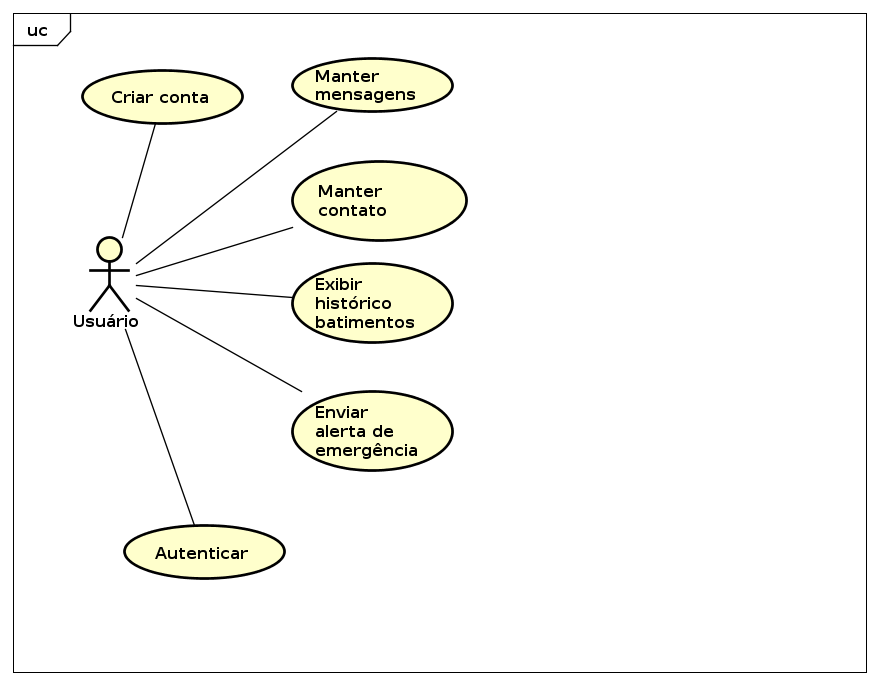
\includegraphics[scale=0.6]{UseCase.png}
	\hfill
\end{figure}
\chapter{Descrição dos casos de uso}
\addcontentsline{arg}{arg}{arg}
%
\subsection{Manter mensagens}
\begin{center}
\begin{tabular}{ |p{7cm}|p{7cm}| } 
 \hline
 \textbf {Nome do caso de uso} & Manter mensagens \\
 \hline
 \textbf{Descrição geral} & Conexão com a internet 24x7 \\
 \hline
 \textbf{Ator Principal} & Usuário comum \\ 
 \hline
 \textbf{Atores Secundários} & Nenhum \\
 \hline
 \textbf{Resumo} & Esse caso de uso tem como finalidade adicionar, excluir, ler ou alterar as mensagens cadastradas pelo usuário. \\
 \hline
 \textbf{Pré-Condições} & O login precisa ter sido realizado\\
 \hline 
 \multicolumn{2}{|c|}{\textbf{Fluxo pricipal de eventos} } \\
 \hline
 \textbf{Ações do ator} & \textbf{Ações do sistema} \\
 \hline
 \multicolumn{2}{|c|}{\textbf{Fluxo de cadastro de mensagens} } \\
 \hline 
 Selecionar cadastrar mensagens & Mostrar tela de cadastro \\
 \hline
 Preencher formulário & \\
 \hline
 Clicar no botão “salvar” & Validar entrada de dados \\
 \hline
  & Salvar dados no banco \\
 \hline
 \multicolumn{2}{|c|}{\textbf{Fluxo de deleção de mensagens} } \\
 \hline 
 Na tela de listagem de mensagens opção excluir mensagem específica & Mostrar tela de confirmação exclusão \\
 \hline
 Confirmar exclusão & Verificar existência da mensagem e em seguida excluir \\
 \hline
 \multicolumn{2}{|c|}{\textbf{Fluxo de edição de mensagens} } \\
 \hline 
 Na tela de listagem, alterar mensagem específica & Exibir tela de alteração de dados \\
 \hline
 Inserir dados a serem alterados & \\
 \hline
 Clicar no botão salvar & Validar as informações a serem alteradas\\
 \hline
  & Tela de confirmação de alteração \\
 \hline
 Confirmar no botão "Sim" & Salvar dados no banco \\
 \hline
 \multicolumn{2}{|c|}{\textbf{Fluxo de listagem de mensagens} } \\
 \hline 
 Na aba mensagens, opção listar mensagens & Buscar dados no banco \\
 \hline
 & Exibir dados\\
 \hline
 \textbf{Pós condições} & Sem pós condições \\
 \hline
 \textbf{Observações} & Se houver inserção de dados inválida pelo usuário neste caso de uso, a aplicação irá exibir uma mensagem de erro\\
 \hline
\end{tabular}
\end{center}
%
\subsection{Manter contatos}
\begin{center}
\begin{tabular}{ |p{7cm}|p{7cm}| } 
 \hline
 \textbf {Nome do caso de uso} & Manter contatos \\
 \hline
 \textbf{Descrição geral} & Caso de uso responsável por manter os contatos os quais receberão alertas de emergência. \\
 \hline
 \textbf{Ator Principal} & Usuário comum \\ 
 \hline
 \textbf{Atores Secundários} & Nenhum \\
 \hline
 \textbf{Resumo} & Esse caso de uso tem como finalidade adicionar, excluir, ler ou alterar os contatos salvos pelo usuário. \\
 \hline
 \textbf{Pré-Condições} & O login precisa ter sido realizado \\
 \hline 
 %-----------------------------------FLUXO DE EVENTOS
 \multicolumn{2}{|c|}{\textbf{Fluxo pricipal de eventos} } \\
 \hline
 \textbf{Ações do ator} & \textbf{Ações do sistema} \\
 \hline
 \multicolumn{2}{|c|}{\textbf{Fluxo de cadastro de contatos} } \\
 \hline 
 Selecionar cadastrar contato & Mostrar tela de cadastro \\
 \hline
 Preencher formulário & \\
 \hline
 Clicar no botão “salvar” & Validar entrada de dados \\
 \hline
  & Salvar dados no banco \\
 \hline
 \multicolumn{2}{|c|}{\textbf{Fluxo de deleção de contatos} } \\
 \hline 
 Na tela de listagem de contatos opção excluir contato específico & Mostrar tela de confirmação exclusão \\
 \hline
 Confirmar exclusão & Verificar existência do contato e em seguida excluir \\
 \hline
 \multicolumn{2}{|c|}{\textbf{Fluxo de edição de contatos} } \\
 \hline 
 Na tela de listagem, clicar em alterar contato & Exibir tela de alteração de dados \\
 \hline
 Escolher contato e clicar no botão editar & Exibir tela de edição \\
 \hline
 Inserir dados a serem alterados & \\
 \hline
 Clicar no botão salvar & Validar as informações a serem alteradas\\
 \hline
  & Tela de confirmação de alteração \\
 \hline
 Confirmar no botão "Sim" & Salvar dados no banco \\
 \hline
 \multicolumn{2}{|c|}{\textbf{Fluxo de listagem de contatos} } \\
 \hline 
 Na aba contatos, opção listar contatos & Buscar dados no banco \\
 \hline
 & Exibir dados\\
 \hline
 \textbf{Pós condições} & Sem pós condições \\
 \hline
 \textbf{Observações} & Se houver inserção de dados inválida pelo usuário neste caso de uso, a aplicação irá exibir uma mensagem de erro\\
 \hline
\end{tabular}
\end{center}
%
\subsection{Exibir histórico de batimentos}
\begin{center}
\begin{tabular}{ |p{7cm}|p{7cm}| } 
 \hline
 \textbf {Nome do caso de uso} & Exibir histórico de batimentos\\
 \hline
 \textbf{Descrição geral} & Exibir um histórico de batimentos cardíacos referente ao usuário \\
 \hline
 \textbf{Ator Principal} & Usuário comum \\ 
 \hline
 \textbf{Atores Secundários} & Nenhum \\
 \hline
 \textbf{Resumo} & Esse caso de uso tem como finalidade exibir uma tela contendo as informações sobre batimentos cardíacos do usuário corrente. \\
 \hline
 \textbf{Pré-Condições} & O login precisa ter sido realizado \\
 \hline 
 %-----------------------------------FLUXO DE EVENTOS
 \multicolumn{2}{|c|}{\textbf{Fluxo pricipal de eventos} } \\
 \hline
 \textbf{Ações do ator} & \textbf{Ações do sistema} \\
 \hline
 \multicolumn{2}{|c|}{\textbf{Fluxo de exibição de histórico} } \\
 \hline 
 Selecionar a opção de visualizar histórico de batimentos & Buscar dados no banco \\
 \hline
  & Mostrar tela de contendo histórico com horário e data de cada item\\
 \hline
 Clicar no botão “salvar” & Validar entrada de dados \\
 \hline
  & Salvar dados no banco \\
 \hline
 \textbf{Pós condições} & Sem pós condições \\
 \hline
 \textbf{Observações} & Se não houver conexão com a internet, a aplicação irá exibir uma mensagem de erro\\
 \hline
\end{tabular}
\end{center}
%
\subsection{Enviar alertas de emergência}
\begin{center}
\begin{tabular}{ |p{7cm}|p{7cm}| } 
 \hline
 \textbf {Nome do caso de uso} & Enviar alertas de emergência\\
 \hline
 \textbf{Descrição geral} & Caso de uso para captação de interação do relógio e envio de mensagem de emergência \\
 \hline
 \textbf{Ator Principal} & Usuário comum \\ 
 \hline
 \textbf{Atores Secundários} & Nenhum \\
 \hline
 \textbf{Resumo} & Caso de uso responsável por captar a interação do usuário com o relógio e enviar uma mensagem para outra pessoa pedindo socorro. \\
 \hline
 \textbf{Pré-Condições} & O login precisa ter sido realizado \\
 \hline 
 %-----------------------------------FLUXO DE EVENTOS
 \multicolumn{2}{|c|}{\textbf{Fluxo pricipal de eventos} } \\
 \hline
 \textbf{Ações do ator} & \textbf{Ações do sistema} \\
 \hline
 \multicolumn{2}{|c|}{\textbf{Fluxo de envio de alerta} } \\
 \hline 
 Apertar uma determinada quantidade de vezes no visor do smartwatch & Buscar dados de contatos no banco \\
 \hline
  & Buscar mensagem de alerta\\
 \hline
 & Preparar mensagem de envio\\
 \hline
 & Enviar requisição de mensagem \\
 \hline
 \textbf{Pós condições} & Nenhuma \\
 \hline
 \textbf{Observações} & Se não houver conexão com a internet, a aplicação irá exibir uma mensagem de erro. Também deve existir ao menos um contato e uma mensagem cadastrados.\\
 \hline
\end{tabular}
\end{center}
%
\subsection{Autenticar usuário}
\begin{center}
\begin{tabular}{ |p{7cm}|p{7cm}| } 
 \hline
 \textbf {Nome do caso de uso} & Autenticar usuário\\
 \hline
 \textbf{Descrição geral} & Caso de uso para permitir acesso na aplicação ao usuário \\
 \hline
 \textbf{Ator Principal} & Usuário comum \\ 
 \hline
 \textbf{Atores Secundários} & Nenhum \\
 \hline
 \textbf{Resumo} & CCaso de uso responsável por fazer a autenticação do usuário na aplicação. \\
 \hline
 \textbf{Pré-Condições} & Necessita de conexão com a internet\\
 \hline 
 %-----------------------------------FLUXO DE EVENTOS
 \multicolumn{2}{|c|}{\textbf{Fluxo pricipal de eventos} } \\
 \hline
 \textbf{Ações do ator} & \textbf{Ações do sistema} \\
 \hline
 \multicolumn{2}{|c|}{\textbf{Fluxo de autenticação} } \\
 \hline 
 Abrir a aplicação & \\
 \hline
 Clicar em login & Exibir tela de login \\
 \hline
 Preencher os campos e submeter & Autenticar o usuário \\
 \hline
 & Exibir tela de sucesso ou erro\\
 \hline
 \textbf{Pós condições} & Nenhuma \\
 \hline
 \textbf{Observações} & Se o usuário ainda não possuir cadastro, receberá a sugestão para que o faça.\\
 \hline
\end{tabular}
\end{center}
%
\subsection{Criar conta}
\begin{center}
\begin{tabular}{ |p{7cm}|p{7cm}| } 
 \hline
 \textbf {Nome do caso de uso} & Criar conta\\
 \hline
 \textbf{Descrição geral} & Caso de uso para permitir cadastro de novos usuário \\
 \hline
 \textbf{Ator Principal} & Usuário comum \\ 
 \hline
 \textbf{Atores Secundários} & Nenhum \\
 \hline
 \textbf{Resumo} & Caso de uso responsável por inserir novos responsáveis na aplicação. \\
 \hline
 \textbf{Pré-Condições} & Nenhuma \\
 \hline 
 %-----------------------------------FLUXO DE EVENTOS
 \multicolumn{2}{|c|}{\textbf{Fluxo pricipal de eventos} } \\
 \hline
 \textbf{Ações do ator} & \textbf{Ações do sistema} \\
 \hline
 \multicolumn{2}{|c|}{\textbf{Fluxo de envio cadastro} } \\
 \hline 
 Abrir a aplicação e clicar cadastrar-se & Apresentar tela de cadastro de usuário \\
 \hline
  Preencher com dados & Verificar se usuário existe no banco de dados\\
 \hline
 & Verificar veracidade de e-mail\\
 \hline
 & Salvar dados do novo usuário no banco \\
 \hline
 & Redirecionar usuário para a tela de boas vindas \\
 \hline
 \textbf{Pós condições} & Nenhuma \\
 \hline
 \textbf{Observações} & Os dados inseridos necessitam ser verídicos, caso contrário será exibida uma tela de erro explicando como contornar.\\
 \hline
\end{tabular}
\end{center}
%
\chapter{Requisitos não funcionais}
\addcontentsline{arg}{arg}{arg}
%---
\begin{center}
\addcontentsline{lot}{table}{What is this doing?}
\begin{tabular}{ |p{7cm}|p{7cm}| }
 \hline
 \textbf{IDRNF} & \textbf{Descrição do requisito não funcional} \\ [0.5ex]
 \hline
 RNF001 & Deve ser feito ao menos um cadastro de usuário \\
 \hline
 RNF002 & Conexão com a internet 24x7 \\
 \hline
 RNF003 & O relógio deve estar sempre bem carregado \\
 \hline
 RNF004 & O relógio deve sempre estar em contato com a pele \\
 \hline
 RNF005 & O usuário deverá integrar somente os relógios aceitos pela aplicação \\
 \hline
 RNF006 & A aplicação deve enviar os dados com rapidez sem necessidade de outras interações
  com o usuário \\
  \hline
 RNF007 & A aplicação deve permitir que o usuário faça o envio da mensagem de emergência com apenas uma ação \\
 \hline
\end{tabular}
\end{center}

\chapter{Diagramas de sequência}
%
\section{Manter mensagem}
\begin{figure}[h]	
	\label{figure_diagrama_sequencia_alterar_mensagem}
	\subsection{Alterar mensagem}
	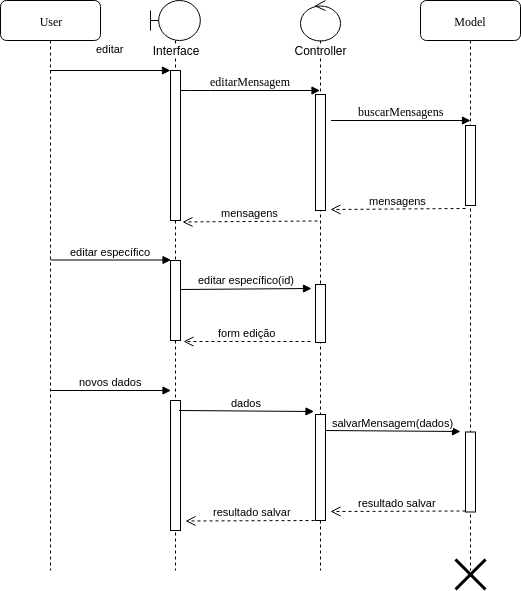
\includegraphics[scale=0.6]{SequenceMensagens/SequenceEditarMensagem.png}
	\caption{Diagrama de sequência: editar mensagens}
	\hfill
\end{figure}
%
\begin{figure}
	\label{figure_diagrama_sequencia_deletar_mensagem}
	\subsection{Deletar mensagem}	
	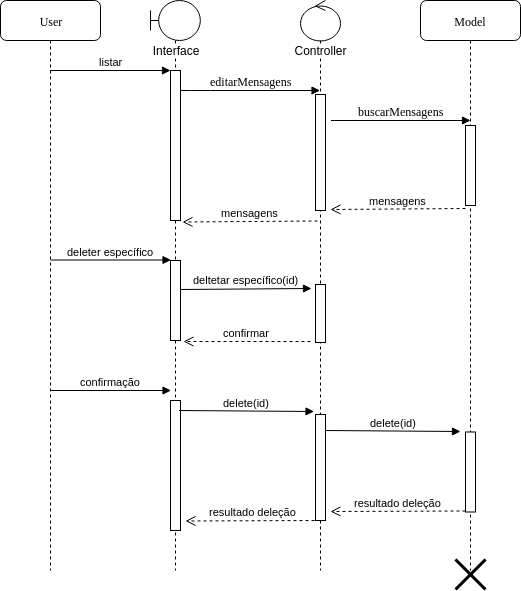
\includegraphics[scale=0.6]{SequenceMensagens/DeleteMessageSequence.png}
	\caption{Diagrama de sequência: deletar mensagens}
	\hfill
\end{figure}
%
\begin{figure}[h]	
	\label{figure_diagrama_sequencia_ver_mensagem}	
	\subsection{Ver mensagem}
	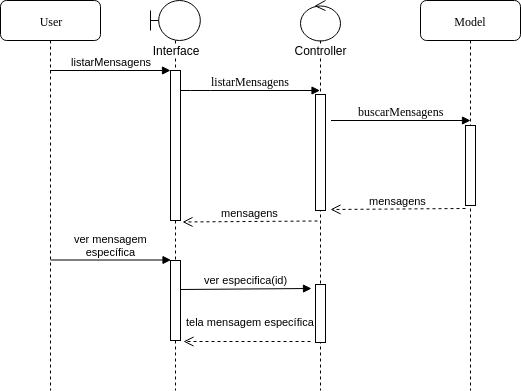
\includegraphics[scale=0.6]{SequenceMensagens/VerMensagensSequence.png}
	\caption{Diagrama de sequência: ver mensagens}
	\hfill
\end{figure}
%
\begin{figure}	
	\label{figure_diagrama_sequencia_criar_mensagem}
	\subsection{Criar mensagem}	
	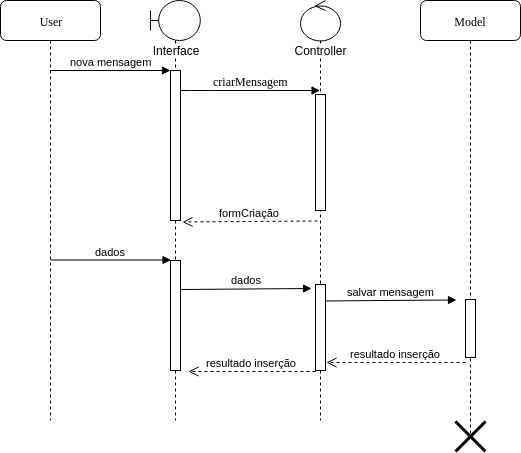
\includegraphics[scale=0.6]{SequenceMensagens/CriarMensagemSequence.png}
	\caption{Diagrama de sequência: adicionar mensagens}
	\hfill
\end{figure}
%
\begin{figure}[h]	
	\label{figure_diagrama_sequencia_enviar_alerta_emergencia}
	\subsection{Enviar alerta de emergência}
	\caption{ Diagrama de sequência: enviar alerta de emergência }
	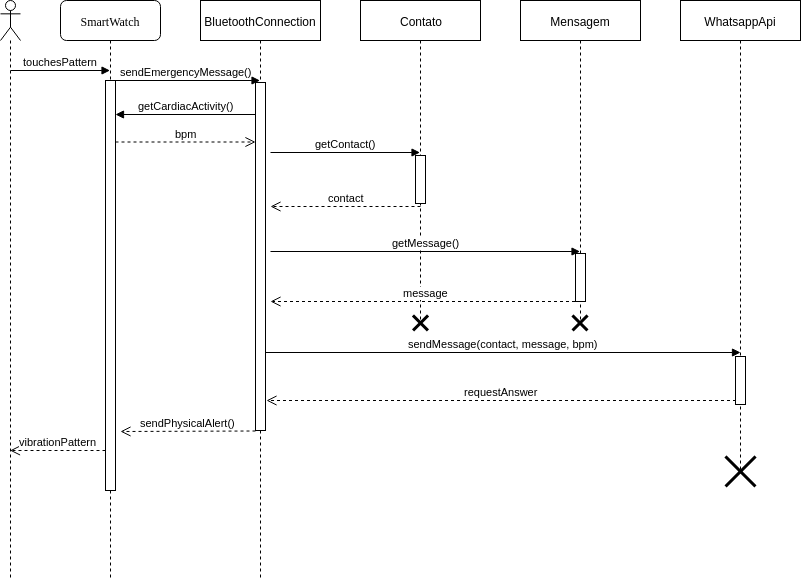
\includegraphics[scale=0.6]{SequenceSmartwatch/Send_Alert.png}
	\hfill
\end{figure}

\chapter{Diagramas de atividades}
\section{Enviar alerta de emergência}	
\begin{figure}[h]	
	\label{figure_diagrama_sequencia_enviar_alerta_emergencia}
	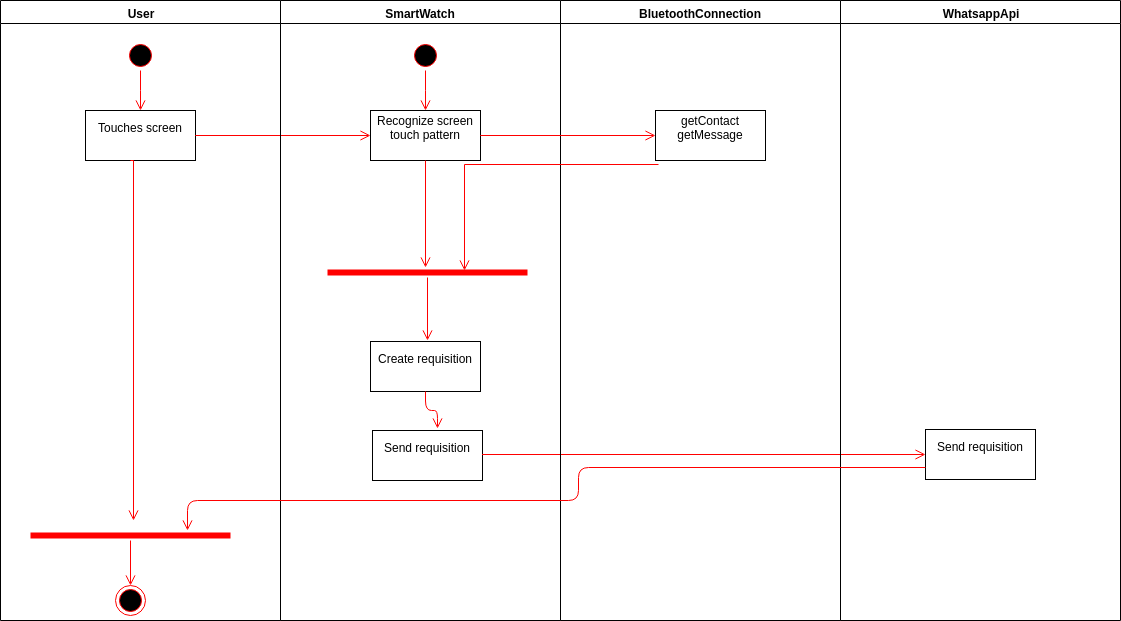
\includegraphics[scale=0.4]{ActivityDiagrams/Send_Message.png}
	\caption{ Diagrama de sequência: enviar alerta de emergência }
	\hfill
\end{figure}
%
\chapter{Diagramas de banco de dados}
\section{Modelo relacional}
\begin{figure}[h]	
	\label{figure_relational_database}	
	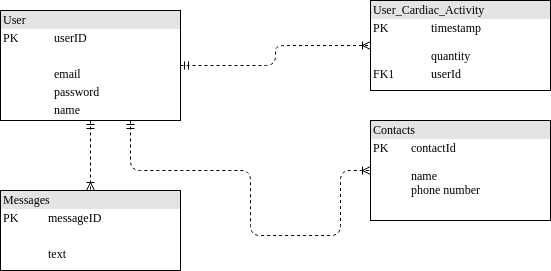
\includegraphics[scale=0.6]{Database/database.png}
	\caption{ Modelo relacional }
	\hfill
\end{figure}
%
\chapter{Interfaces de usuário}
\section{Histórico de batimentos cardíacos}
\begin{figure}[h]	
	\label{figure_cardiac_activity_history}	
	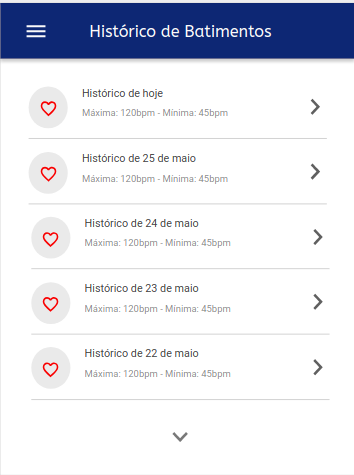
\includegraphics[scale=0.8]{interfaces/cardiac_history.png}
	\caption{ Histórico de batimentos cardíacos }
	\hfill
\end{figure}
%
\chapter{Cronograma do projeto}
% ---
% Conclusão
% ---
\chapter{Conclusão}
\addcontentsline{arg}{arg}{arg}
% ---

% ----------------------------------------------------------
% ELEMENTOS PÓS-TEXTUAIS
% ----------------------------------------------------------
\postextual
% ----------------------------------------------------------

% ----------------------------------------------------------
% Referências bibliográficas
% ----------------------------------------------------------
\chapter{Referências bibliográficas}
\addcontentsline{arg}{arg}{arg}

% ----------------------------------------------------------
% Glossário
% ----------------------------------------------------------
%
% Consulte o manual da classe abntex2 para orientações sobre o glossário.
%
%\glossary

% ----------------------------------------------------------
% Apêndices
% ----------------------------------------------------------

% ---
% Inicia os apêndices
% ---


% ----------------------------------------------------------
% Anexos
% ----------------------------------------------------------

% ---
% Inicia os anexos
% ---


%---------------------------------------------------------------------
% INDICE REMISSIVO
%---------------------------------------------------------------------
\phantompart
\printindex
%---------------------------------------------------------------------

\end{document}
